% Some classes load the `subfigure` package which clashes with
% our internal use of `subfig` for subfloats. We are most likely
% not going to need the canned subfigure functionality anyways,
% so we'll trick LaTeX into thinking it already loaded `subfigure`
\makeatletter
\newcommand{\dontusepackage}[2][]{%
  \@namedef{ver@#2.sty}{9999/12/31}%
  \@namedef{opt@#2.sty}{#1}}
\makeatother
\dontusepackage{subfigure}
%
\documentclass[]{segabs}
\usepackage{amssymb,amsmath,amsbsy,bm}
\usepackage{fixltx2e} % provides \textsubscript
% use upquote if available, for straight quotes in verbatim environments
\IfFileExists{upquote.sty}{\usepackage{upquote}}{}
\usepackage[T1]{fontenc}
\usepackage[utf8]{inputenc}
% use microtype if available
\IfFileExists{microtype.sty}{\usepackage{microtype}}{}
\usepackage{natbib}
\bibliographystyle{seglike}
\usepackage{listings}
% Define slightly more reasonable Listings defaults
\lstset{
    basicstyle=\ttfamily\small,
    breaklines=true,
    prebreak=\raisebox{0ex}[0ex][0ex]{\ensuremath{\hookleftarrow}},
    frame=lines,
    showtabs=false,
    showspaces=false,
    showstringspaces=false,
    keywordstyle=\color[gray]{0.4}\bfseries,
    commentstyle=\color[gray]{0.65}\itshape,
    numbers=left,
    captionpos=b,
}
\usepackage{longtable,booktabs}
\usepackage{graphicx}
% Redefine \includegraphics so that, unless explicit options are
% given, the image width will not exceed the width of the page.
% Images get their normal width if they fit onto the page, but
% are scaled down if they would overflow the margins.
\makeatletter
\def\ScaleIfNeeded{%
  \ifdim\Gin@nat@width>\linewidth
    \linewidth
  \else
    \Gin@nat@width
  \fi
}
\makeatother
\let\Oldincludegraphics\includegraphics
{
 \catcode`\@=11\relax
 \gdef\includegraphics{\@ifnextchar[{\Oldincludegraphics}{\Oldincludegraphics[width=\ScaleIfNeeded]}}
}
\usepackage{caption}
\usepackage{float}
% Override extremely conservative LaTeX float placement rules
% (might need to be removed for "manuscript" styles)
\renewcommand{\topfraction}{0.85}	% max fraction of floats at top
\renewcommand{\bottomfraction}{0.75}	% max fraction of floats at bottom
\setcounter{topnumber}{2}
\setcounter{bottomnumber}{2}
\setcounter{totalnumber}{4}
\setcounter{dbltopnumber}{2}    % for 2-column pages
\renewcommand{\dbltopfraction}{0.85}	% fit big float above 2-col. text
\renewcommand{\textfraction}{0.10}	% allow minimal text w. figs
\renewcommand{\floatpagefraction}{0.85}	% require fuller float pages
\renewcommand{\dblfloatpagefraction}{0.85}	% require fuller float pages
% Encourage floats to be placed in the vacinity of where it is defined
% (in some manuscript styles where figures are collected at the end, the 'h'
% option might need to be removed by a separate '\floatplacement' call in the
% 'header-includes' metadata field)
\floatplacement{figure}{htbp}
\floatplacement{scholmdAlgorithm}{htbp}
\floatplacement{table}{htbp}
\usepackage{subfig}
\captionsetup[subfloat]{margin=1em}
\usepackage{algorithm} % <- from the `algorithms` package
% Rename the `algorithm` float environment so that it doesn't
% conflict with the one provided by `algorithm2e`, which is
% also called `algorithm`. The following environments are renamed:
%       algorithm -> scholmdAlgorithm
%       algorithm* -> scholmdAlgorithm*
%       listofalgorithms -> scholmdListofalgorithms
\let\scholmdAlgorithm\algorithm
\let\endscholmdAlgorithm\endalgorithm
\let\algorithm\relax \let\endalgorithm\relax
\let\scholmdListofalgorithms\listofalgorithms
\let\listofalgorithms\relax
{
 \catcode`\*=11\relax
 \global\let\scholmdAlgorithm*\algorithm*
 \global\let\endscholmdAlgorithm*\endalgorithm*
 \global\let\algorithm*\relax 
 \global\let\endalgorithm*\relax
}


\usepackage[unicode=true]{hyperref}
\hypersetup{breaklinks=true,
            bookmarks=true,
            pdfauthor={},
            pdftitle={Extreme low memory seismic inversion via matrix sketching.},
            colorlinks=true,
            citecolor=black,
            urlcolor=blue,
            linkcolor=black,
            pdfborder={0 0 0}}
\urlstyle{same}  % don't use monospace font for urls
\setlength{\emergencystretch}{3em}  % prevent overfull lines

\title{Extreme low memory seismic inversion via matrix sketching.}
\author{Mathias Louboutin\textsuperscript{1}, Felix J.
Herrmann\textsuperscript{1}\\\textsuperscript{1}School of Computational
Science and Engineering, Georgia Institute of Technology\\}
\date{}

\begin{document}
\maketitle




\section{Summary}\label{summary}

\{\textgreater{}\textgreater{} Redo all figures as individual ones with
subfigures and captions in markown\textless{}\textless{}\}

\section{Introduction}\label{introduction}

\begin{itemize}
\item
  \citet{louboutin2015segtcs}
\item
  \citet{witte2018cls}, bp ref, chvron ref
\item
  checkpointing (griewank, symes navjot)
\item
  Mengmeng EV
\item
  Implemented on top of JUDI \citep{witte2018alf} using Devito for the
  wave equations propagators
  \citep[\citet{devito-compiler}]{devito-api}. Thanks to Devito's
  flexibility and JUDI's separation of concern, we can easily run the
  inversion with our memory efficient method on GPU with the same code
  adding a single flag.
\end{itemize}

\section{Theory}\label{theory}

We consider the standard adjoint-state FWI problem that aims a
minimizing the difference between field recorded data and numerically
modelled synthetic data in a least-square sense\citep[\citet{tarantola},
\citet{virieux}, \citet{louboutin2017fwi},
\citet{louboutin2017fwip2}]{lionsjl1971}. This data fitting problem is
defined as:
%
\begin{equation}
\underset{\mathbf{m}}{\operatorname{minimize}} \ \frac{1}{2} ||\mathbf{F}(\mathbf{m}; \mathbf{q}) - \mathbf{d}_{obs} ||_2^2
\label{adj}
\end{equation}
%
 where $\mathbf{m}$ is the physical model parameter (squared slowness in
the isotropic acoustic case), $\mathbf{q}$ is the source,
$\mathbf{d}_{obs}$ is the observed data and $\mathbf{F}$ is the forward
modeling operator. This data misfit is usually minimized using
gradient-based optimization methods such as gradient descent
\citep{plessixasfwi} or gauss-newton {[}maybe xiangli ref{]} are
necessary. In this work, we propose an unbiased estimate of that
gradient, which means that that estimate equals the FWI gradient in
expectation. In the following section, we describe our proposed method
in the isotropic acoustic case.

\subsection{Adjoint state gradient}\label{adjoint-state-gradient}

In the isotropic acoustic approximation of the physics, the gradient of
the data misfit objective function~\ref{adj} is defined as
\citep{haber10tremp}:
%
\begin{equation}
\mathcal{I} = \sum_t \frac{d^2 \mathbf{u}}{dt^2}(t) \mathbf{v}(t)
\label{iccc}
\end{equation}
%
 where $\mathbf{u}, \mathbf{v}$ are the forward and adjoint wavefields
solutions of the forward and adjoint wave equations. Following standard
linear algebra, this zero-lag correlation over time can be rewritten as
the trace of an outer product for each point $\mathbf{x}$ in space as
follows.
%
\begin{equation}
\mathcal{I}(\mathbf{x}) = \text{tr}(\mathbf{u}(\mathbf{x})\mathbf{v}(\mathbf{x})^\top).
\label{optr}
\end{equation}
%
 This outer product is in practice not feasible to compute as each point
in space requires an $n_t x n_t$ matrix, with $n_t$ the number of
computational time steps. Computing this outer product woudl therefore
require $n_t$ more memory than standard FWI. To tackle this memory
bottleneck, we instead compute this trace via matrix probing {[}format
probing refs{]}. Matrix probing is a method that provides information
about a matrix, in this case the trace, via matrix vector products when
the matrix itself is either unknwn or too expensive to compute. The
trace estimation of our outer product wrties as follows:
%
\begin{equation}
\begin{split}
    \tilde{\mathcal{I}}(\mathbf{x}) = \frac{1}{N} \sum_{i=1}^{N} \mathbf{z}_i^\top \mathbf{u}(\mathbf{x})\mathbf{v}(\mathbf{x})^\top \mathbf{z}_i \\
    \text{ s.t } \mathbb{E}(\mathbf{z}_i^\top \mathbf{z}_i) = 1, \mathbb{E}(\mathbf{z}_i) = 0,
\end{split}
\label{trpr}
\end{equation}
%
 or in its matrix form:
%
\begin{equation}
\begin{split}
    \tilde{\mathcal{I}}(\mathbf{x}) = \frac{1}{N} \text{tr}(\mathbf{Z}^\top \mathbf{u}(\mathbf{x}) \mathbf{v}(\mathbf{x})^\top \mathbf{Z}) \\
\end{split}
\label{trprM}
\end{equation}
%
 where $\mathbf{Z}$ is the matrix with each $\mathbf{z}_i$ in its
column. We will discuss the importance of the choice for these probing
vectors $\mathbf{z}_i$ in a subsequent section. This probing, unlike
computing the trace, does not require to compute the outer product but
only matrix vector products that can be made extremely memory scheduling
the computation accross the forward and adjoint propagation. In the
above Equation~\ref{trpr}, that memory optimal schedule is:

\begin{itemize}
\item
  \begin{enumerate}
  \def\labelenumi{\arabic{enumi}.}
  \itemsep1pt\parskip0pt\parsep0pt
  \item
    $u_z = \mathbf{Z}^\top \mathbf{u}(\mathbf{x})$
  \end{enumerate}
\item
  \begin{enumerate}
  \def\labelenumi{\arabic{enumi}.}
  \itemsep1pt\parskip0pt\parsep0pt
  \item
    $v_z = \mathbf{v}(\mathbf{x})^\top \mathbf{Z} $
  \end{enumerate}
\item
  \begin{enumerate}
  \def\labelenumi{\arabic{enumi}.}
  \setcounter{enumi}{2}
  \itemsep1pt\parskip0pt\parsep0pt
  \item
    $\tilde{\mathcal{I}}(\mathbf{x}) = \text{tr}(u_z v_z)$.
  \end{enumerate}
\end{itemize}

Through these three steps, we obtain the unbiased {[}refs{]} estimate of
the true update $\mathbb{E}(\tilde{\mathcal{I}}) = \mathcal{I}$ that
only requires randomized accumulation of the wavefields during their
respective propagation. These three memory-optimal steps can then be
merged with the time-stepper to implement efficient on-the-fly matrix
probing, summarized in algorithm~\ref{pic}.

\begin{scholmdAlgorithm}
\textbf{for~t=1:nt}\\1.~$\mathbf{u}(t+1) = f(\mathbf{u}(t), \mathbf{u}(t-1), \mathbf{m}, \mathbf{q})$\\2.~$u_z(\mathbf{x}) += \mathbf{Z}^\top \mathbf{u}(t, \mathbf{x})$\\\textbf{for~t=nt:1}\\1.~$\mathbf{v}(t-1) = f^\top(\mathbf{v}(t), \mathbf{v}(t+1), \mathbf{m}, δ \mathbf{d})$\\2.~$v_z(\mathbf{x}) += \mathbf{v}(t, \mathbf{x})^\top \mathbf{Z}$\\$\tilde{\mathcal{I}}(\mathbf{x}) = \text{tr}(u_z v_z)$
\caption{Seismic inversion via probed trace estimation where $f, f^\top$
are the forward and backward time-stepping operators.}\label{pic}
\end{scholmdAlgorithm}

We compute our estimate for varying probing sizes and compare it to the
true gradient on Figure \#2d-grad~. We show the probed estimate for
varying number of probing vectors and the difference with true gradient.
W ca clearly see that the accuracy increases wit the number of probing
vectors and that we alread obtain an good approximation with as little
as 16 to 32 vectors.

\begin{figure}
\centering
\captionsetup[subfigure]{labelformat=empty}
\subfloat[]{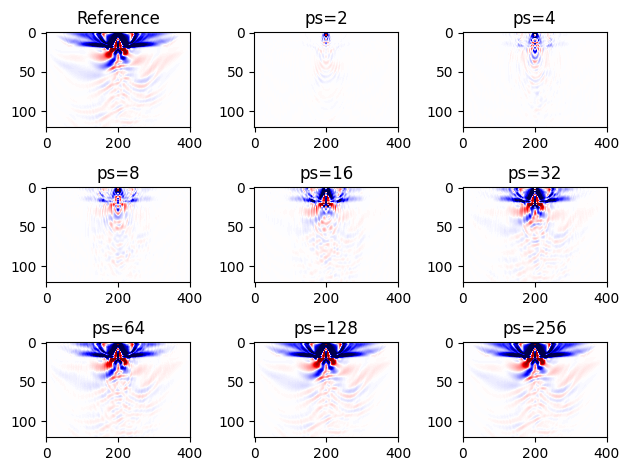
\includegraphics[width=1.000\hsize]{./figures/Probed_grad.png}}
\\
\subfloat[]{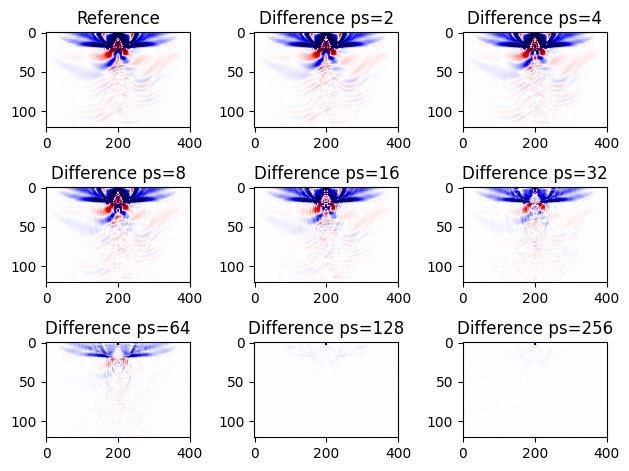
\includegraphics[width=1.000\hsize]{./figures/Probed_err.png}}
\caption*{Single source gradient and unbiased estimates for varying
probing sizes.}
\end{figure}

With this few probing vector, we obtain massive memory reduction
compared to conventional FWI whith a very small computationnal overhead
(near negligeable in theory). We now detail the exact memory savings.

\subsection{Memory estimates}\label{memory-estimates}

From this formulation, we can estimate the memory imprint of our method
compared to conventional FWI. For completeness, we also consider other
mainstream low memory methods: optimal checkpointing {[}refs{]},
boundary methods {[}refs{]}, and DFT methods \citep{witte2018cls}. This
memory overview generalizes to other wave-equations and imaging
conditions easily as our method generalizes to any adjoint-state,
zero-lag cross-correlation. We estimate the memory requirements for a
three-dimensional domain with $N_x N_y N_z$ grid points and $n_t$ time
steps. Conventional FWI requires to save the full time-space forward
wavefield to compute the gradient. This requirement leads to a memory
requirement of $N n_t$ floating point values of memory in single
precision. Our method, on the other hand, for $p_s$ probing vector (i.e
$\mathbf{Z} \in \mathbb{R}^{n_t \times p_s}$), requires $N p_s$ floating
point values in the forward pass and $N p_s$ in the backward pass for a
total of $2 N p_s$ value. The memory reduction factor is therefore
$\frac{n_t}{2 p_s}$. This memory reduction is similar to computing the
gradient with $p_s$ Fourier modes, i.e on-the-fly Fourier
\citep{witte2018cls}. We summarize the memory usage compared to
state-of-the-art algorithms in table~\ref{memest}.

\begin{table}
\centering
\begin{tabular}{cccccc}
\toprule\addlinespace
& FWI & DFT & Probing & Optimal checkpointing & Boundary
reconstruction\tabularnewline
\midrule
Compute & 0 & $\mathcal{O}(100) n_t N$ & $\mathcal{O}(10) n_t N$ &
$\mathcal{O}(log(n_t)) N n_t$ & $n_t N$\tabularnewline
Memory & $N n_t $ & $\mathcal{O}(10) N$ & $\mathcal{O}(10) N$ &
$\mathcal{O}(10) N$ & $n_t N^{\frac{2}{3}}$\tabularnewline
\bottomrule
\end{tabular}
\caption{Memory estimates and computational overhead of different
seismic inversion methods for $n_t$ time steps and $N$ grid
points.}\label{memest}
\end{table}

It is worth noting that unlike the other methods in the table, boundary
reconstruction methods tend to have stability issues for more complex
physics, in particular with physical attenuation making it ill-suited
for real-world applications.

\subsection{Imaging condtions}\label{imaging-condtions}

In some cases, such as reverse-time migration (RTM) or to add eemphasis
to a certain range of wavenumber for FWI, an imaging condtion may be
applied to the forward and adjoint wavefield instead of using the
adjoint state gradient. Usually, these imaging condition can be
expressed as linear operators that only act on the spatial dimension fo
the wavefields. Because such operators are linear and independent of
times, we can factor them out and directl apply them to the probed
vectors rather than at every time steps. This property can be seen from
rewriting Equation~\ref{trpr} as:
%
\begin{equation}
    \tilde{\mathcal{I}}(\mathbf{x}) = \frac{1}{N} \sum_{i=1}^{N} \left [ \sum_{t=1}^{n_t} (\mathbf{z}_i(t) \mathbf{u}(t, \mathbf{x})) \sum_{t=1}^{n_t}(\mathbf{v}(t, \mathbf{x}) \mathbf{z}_i(t)) \right ]
\label{trpr_t}
\end{equation}
%
 and for any linear operators $\mathbf{D}_u$ we have
%
\begin{equation}
\sum_{t=1}^{n_t} \mathbf{z}_i(t) \mathbf{D}_u(\mathbf{u}(t, \mathbf{x})) = \mathbf{D}_u(\sum_{t=1}^{n_t} (\mathbf{z}_i(t) \mathbf{u}(t, \mathbf{x}))).
\label{lint}
\end{equation}
%
 This property makes our probing method extremely advantageous as these
imaging operations can be as expensive as an extra PDE if applied at
every time steps while we only need to apply them $\mathcal{O}(10)$
times.

\subsection{Probing vectors}\label{probing-vectors}

In order to make our method very efficient, the choice of probing
vectors $\mathbf{z}_i$ is crucial. In its most simple formulation, this
matrix probing method only requires random vectors from the normal
distribution $\mathbf{z}_i \in \mathbb{N}(0, 1)$ or the Radamaecher
distribution (random $\pm 1$) {[}refs{]}. However, matrix probing with
these vectors has fairly low convergence rate and requires large number
of probing vectors ($N >> 1$). To improve the estimate, {[}ref{]}
proposed to compute a QR decomposition of the range of the matrix to be
probed
$\mathbf{Z} = QR(\mathbf{u}(\mathbf{x})\mathbf{v}(\mathbf{x})^\top S)$
with $S$ an $n_t \times N$ matrix of $± 1$. In theory, this QR
factorization greatly improves the estimation \citep{refs}. However,
computing a QR factorization for each subsurface point would be
unfeasible. As a proxy for the outer product of the wavefields, we
compute a single probing matrix for the entire subsurface based on the
observed data $Z = QR(\mathbf{d}_{obs}\mathbf{d}_{obs}^\top S)$ since
the data is the restriction of a wavefield.

We show what the probing vectors look like on Figure \#pvec. It is of
importance that these vectors are orthonormal but do not form a basis.
They satisfy $\mathbf{Z} \mathbf{Z}^\top = I$ but
$\mathbf{Z}^top \mathbf{Z} \neq I$ is a low rank approximation of
$\mathbf{d}_{obs} \mathbf{d}_{obs}^\top$ as shown on Figure~\ref{pvec}.
This sets our method apart from transform domain methods such as
on-the-fly DFT that can be interpreted as probing methods where the
probing vectors are a subset of the Fourier basis.

\begin{figure}
\centering
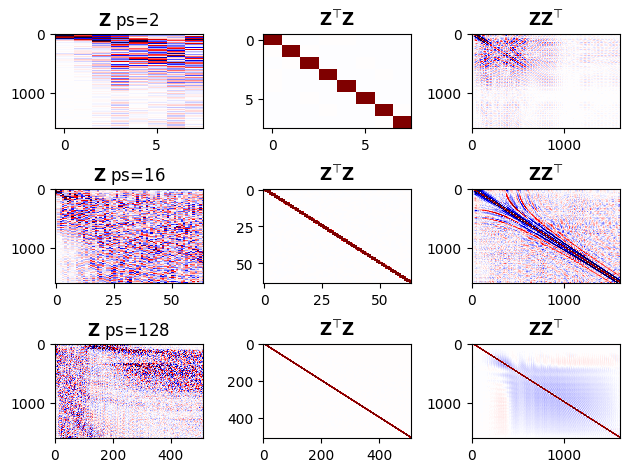
\includegraphics[width=1.000\hsize]{./figures/Zi.png}
\caption{Probing vector for varying probing size.}\label{pvec}
\end{figure}

\section{Example}\label{example}

We illustrate our method on the 2D overthrust model and compare our
inversion results to conventional FWI and on-the-fly DFT. The model is
20km by 5km isotropic acoustic. The dataset consists of 97 sources at
50m depth and 127 ocean bottom nodes (500m depth) 50m apart. The source
function is an 8Hz Ricker wavelet. We show the true model and the
initial background model on Figure \#2d-setuo.

\begin{figure}
\centering
\includegraphics[width=1.000\hsize]{./figures/init.png}
\caption*{True (top) and initial (bottom) velocity models for
inversion.}
\end{figure}

In all the experiments presented here, we ran 20 iteration of spectral
projected gradient (gradient descent with box constraints)
\citep{minconf} with 20 randomly selected shots per iteration {[}felix
ref{]}.

\begin{figure}
\centering
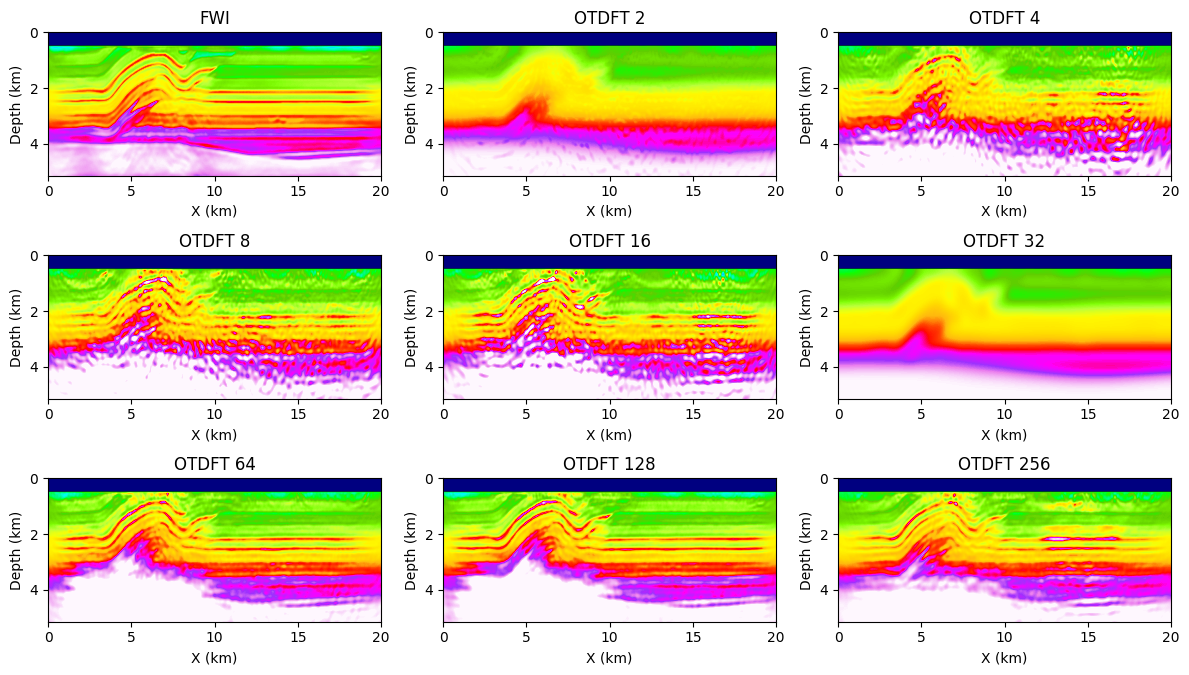
\includegraphics[width=1.000\hsize]{./figures/DFT_fwi.png}
\caption*{FWI on the 2D overthrust model with varying number of probing
vectors.}
\end{figure}

\begin{figure}
\centering
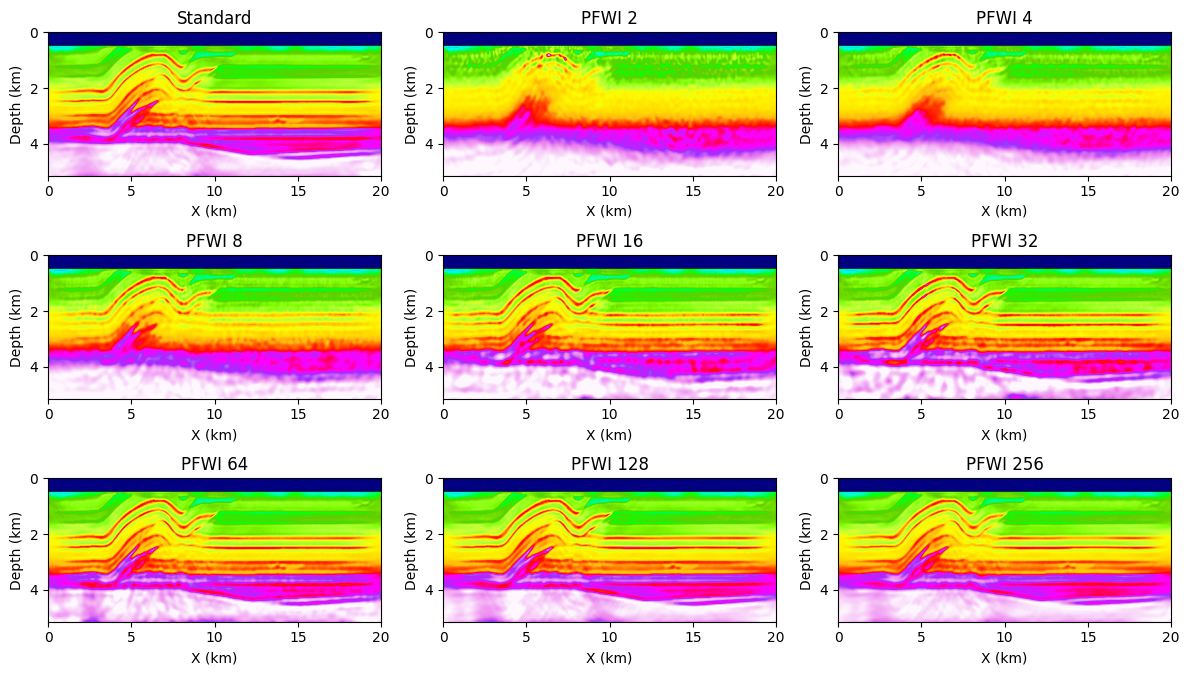
\includegraphics[width=1.000\hsize]{./figures/probed_fwi.png}
\caption*{FWI on the 2D overthrust model with varying number of probing
vectors.}
\end{figure}

\begin{figure}
\centering
\captionsetup[subfigure]{labelformat=empty}
\subfloat[]{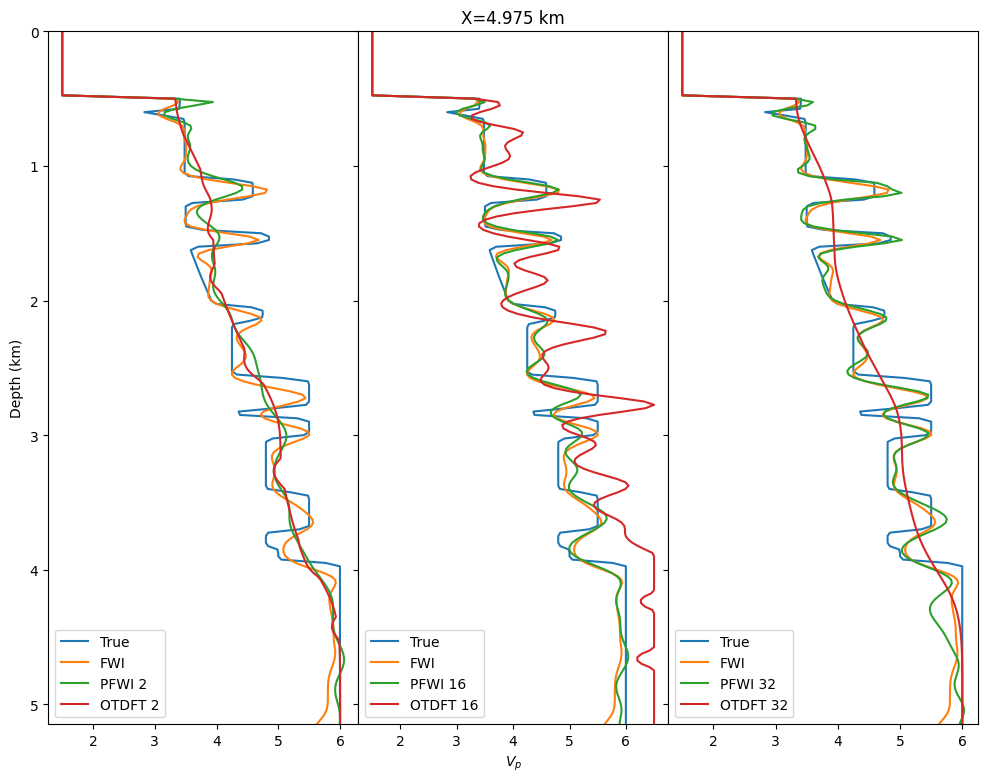
\includegraphics[width=0.330\hsize]{./figures/vertical_trace_200_select.png}}
\subfloat[]{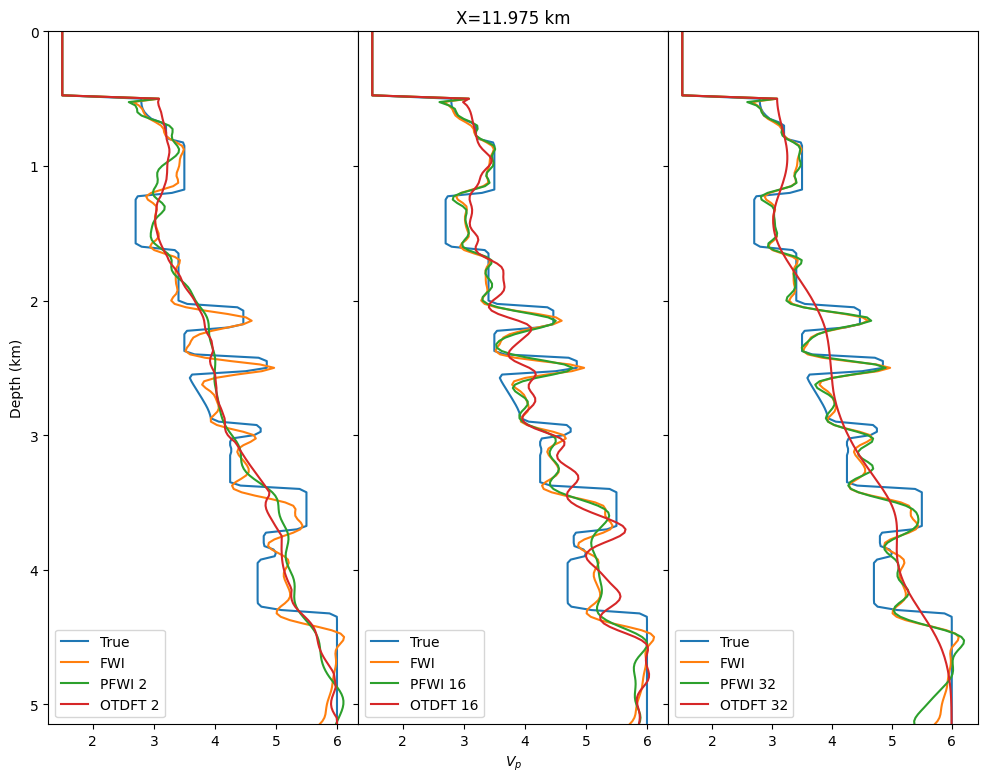
\includegraphics[width=0.330\hsize]{./figures/vertical_trace_480_select.png}}
\subfloat[]{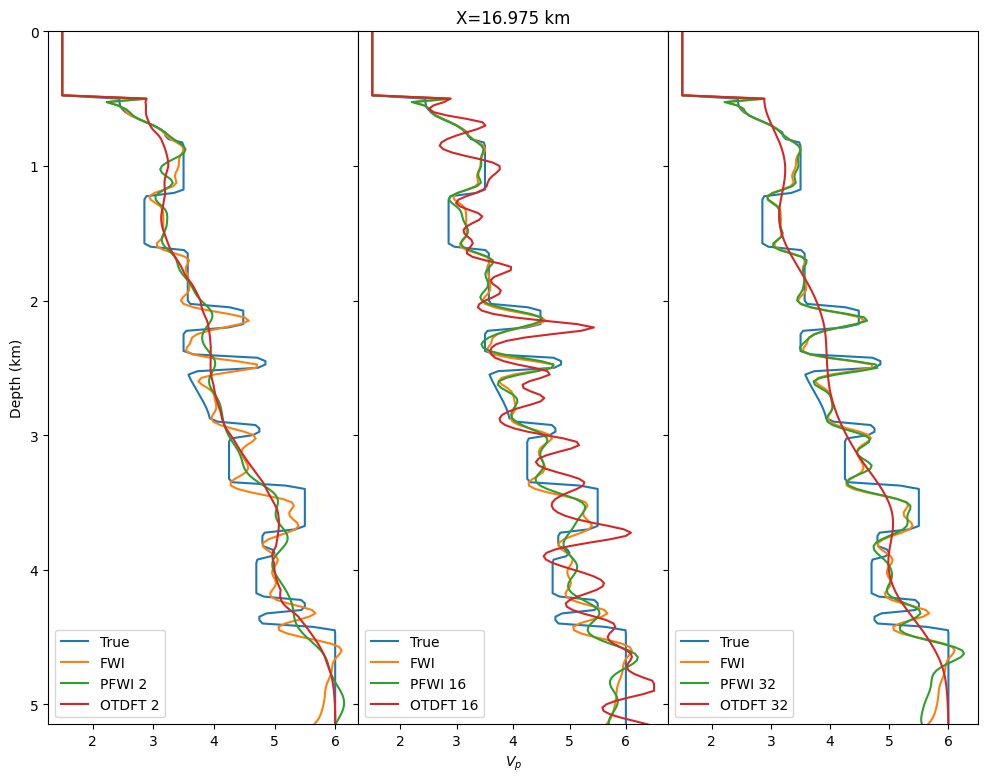
\includegraphics[width=0.330\hsize]{./figures/vertical_trace_680_select.png}}
\caption*{Vertical trace comparison between the true model, standard
FWI, on-the-fly DFT and time probing.}
\end{figure}

\section{Discussion and Conclusions}\label{discussion-and-conclusions}

\section{References}\label{references}

\bibliography{bibliography}

\end{document}
